% ====================== CONTENT FILE — CipherCorgi Poster (Portrait White) ===========================

% ---- Poster colors ----
\def\postercolor{white}
\def\backgroundcolortitle{ETHBlue}
\def\backgroundcolorcolor{verylightblue}
\def\backgroundcolorwhite{verylightgray}
\def\linecolor{verylightgray}

% ---- Department ----
\def\department{\linespread{1.1}%
\Large Dept.\ of Computer Science,\\
Interactive AI, ETH Z\"urich
}

% ---- Title ----
\def\title{%
\VERYHuge \white {\bf
Exploring Simulated Web Agents vs Real User Journeys
}\\[20pt]}

% ---- Authors ----
\def\authors{\LARGE Kaan Bayraktar, Florian F\"org, Elif \"Ozsoy, Haroldas Plytnikas}

% ---- Affiliations ----
\def\affiliations{\LARGE Interactive AI \& Visualisations, ETH Z\"urich}

% ---- Partners ----
\def\partner{%
\vspace{3mm}\hspace{0.5cm}%
\Large\color{ETH6}
Interactive AI Course $\cdot$ ETH Z\"urich $\cdot$ 2026}


% ====================== 1. INTRODUCTION = Goal & Motivation ===================
\def\introtext{%
{\large \black
{\Large\bf We propose a framework for UX designers to scale UX evaluation,
replacing the slow data collection loop with aligned web agents.}\\[14pt]

{\bf $\bullet$\ Scale UX evaluation}\\[4pt]
Reduce slow human testing cycles by running AI agents on the same tasks in parallel.\\[10pt]

{\bf $\bullet$\ Compare AI vs.\ human navigation}\\[4pt]
Identify where agents and users diverge, surfacing friction points that take weeks to uncover manually.\\[10pt]

{\bf $\bullet$\ Human-in-the-loop re-evaluation}\\[4pt]
Make changes, re-run agents. Version-stamped journeys enable before/after comparison.
}%
}


% ====================== 2. METHOD OVERVIEW = Users + Data + Workflow ==========
\def\methodtext{%
{\large \black
{\Large\bf Users}\\[4pt]
{\bf $\bullet$\ UX designers \& Web developers}\\[3pt]
Evaluating and improving web interfaces. Validating navigation flows and detecting usability issues.\\[12pt]

{\Large\bf Data}\\[4pt]
{\bf $\bullet$\ Human User Journeys}\\[3pt]
Collected via reverse proxy distributed to real testers. Every click, scroll, and navigation recorded per task.\\[8pt]

{\bf $\bullet$\ Web Agent Journeys}\\[3pt]
AI browser sessions running the same tasks. Full step history with per-step screenshots.\\[8pt]

{\bf $\bullet$\ Collected per step}\\[3pt]
Clicks $\cdot$ Scrolls $\cdot$ Screenshots $\cdot$ Timestamps $\cdot$ URLs $\cdot$ Task descriptions\\[12pt]

% {\Large\bf Workflow \& Interaction}\\[4pt]
% \textbf{1.~Setup:} Host website, configure proxy, define tasks.\\[3pt]
% \textbf{2.~Data Collection:} Gather human and AI journey data in parallel.\\[3pt]
% \textbf{3.~Analysis:} LLM comparative analysis surfaces ranked pain points.\\[3pt]
% \textbf{4.~Reconfiguration:} Update the website based on insights.\\[3pt]
% \textbf{5.~Re-Evaluate:} Re-run agents steered by previously gathered human journeys.
}%
}


% ====================== 3. MATERIALS = Action Points Dashboard ================
\def\materialstext{%
\begin{center}
\scalebox{0.55}{%
\begin{tikzpicture}[x=1cm, y=1cm,
  marrow/.style={
    ->, line width=0.18cm, color=CCblue,
    -{Stealth[length=0.55cm, width=0.42cm]}
  },
  badge/.style={
    rectangle, rounded corners=0.35cm,
    fill=CCbluesoft, text=CCblue,
    font=\large\bfseries,
    inner xsep=0.45cm, inner ysep=0.18cm
  },
  annot/.style={font=\large, text=CCsec, align=center},
]
\begin{scope}[xshift=-38cm, yshift=-1cm]

% ── Sub-view cards (bottom row) ───────────────────────────────

% -- Journey Flows (Sankey) --
\begin{scope}
  \clip[rounded corners=0.5cm] (38.5,0.5) rectangle (50,24);
  \fill[CCbluesoft!80!white] (38.5,22.3) rectangle (50,24);
  \fill[white] (38.5,0.5) rectangle (50,22.3);
\end{scope}
\draw[rounded corners=0.5cm, draw=CCborder, line width=0.05cm]
  (38.5,0.5) rectangle (50,24);
\foreach \dx in {1.0, 1.65, 2.3} {
  \fill[CCblue!50!white] (38.5+\dx, 23.15) circle (0.15cm);
}
\node[annot, text=CCborder, font=\large] at (44.25,12.5)
  {\textit{Sankey / Flow}};
\node[font=\large\bfseries, text=CCblue] at (44.25,24.7)
  {Journey Flows};
\node[annot, font=\normalsize] at (44.25,-0.2)
  {Step-by-step path divergence};

% -- Click Heatmaps --
\begin{scope}
  \clip[rounded corners=0.5cm] (51,0.5) rectangle (62.5,24);
  \fill[CCbluesoft!80!white] (51,22.3) rectangle (62.5,24);
  \fill[white] (51,0.5) rectangle (62.5,22.3);
\end{scope}
\draw[rounded corners=0.5cm, draw=CCborder, line width=0.05cm]
  (51,0.5) rectangle (62.5,24);
\foreach \dx in {1.0, 1.65, 2.3} {
  \fill[CCblue!50!white] (51+\dx, 23.15) circle (0.15cm);
}
\node[annot, text=CCborder, font=\large] at (56.75,12.5)
  {\textit{Heatmap}};
\node[font=\large\bfseries, text=CCblue] at (56.75,24.7)
  {Click Heatmaps};
\node[annot, font=\normalsize] at (56.75,-0.2)
  {Density overlay per screenshot};

% -- Human vs. AI --
\begin{scope}
  \clip[rounded corners=0.5cm] (63,0.5) rectangle (73,24);
  \fill[CCbluesoft!80!white] (63,22.3) rectangle (73,24);
  \fill[white] (63,0.5) rectangle (73,22.3);
\end{scope}
\draw[rounded corners=0.5cm, draw=CCborder, line width=0.05cm]
  (63,0.5) rectangle (73,24);
\foreach \dx in {1.0, 1.65, 2.3} {
  \fill[CCblue!50!white] (63+\dx, 23.15) circle (0.15cm);
}
\node[annot, text=CCborder, font=\large] at (68,12.5)
  {\textit{Human vs.\ AI}};
\node[font=\large\bfseries, text=CCblue] at (68,24.7)
  {Human vs.\ AI};
\node[annot, font=\normalsize] at (68,-0.2)
  {Linked trajectory comparison};

% ── Arrows from main Action Points card to sub-views ──────────
\draw[marrow, line width=0.12cm] (44.25,25.5) -- (44.25,24.3);
\draw[marrow, line width=0.12cm] (56.75,25.5) -- (56.75,24.3);
\draw[marrow, line width=0.12cm] (68,25.5)    -- (68,24.3);

% ── Main Action Points card ───────────────────────────────────
\begin{scope}
  \clip[rounded corners=0.6cm] (38.5,25.5) rectangle (73,45.5);
  \fill[CCblue] (38.5,43.8) rectangle (73,45.5);
  \fill[CCbg!60!white] (38.5,25.5) rectangle (73,43.8);
\end{scope}
\draw[rounded corners=0.6cm, draw=CCborder, line width=0.06cm]
  (38.5,25.5) rectangle (73,45.5);
\foreach \dx in {1.1, 1.8, 2.5} {
  \fill[white!60!CCblue] (38.5+\dx, 44.65) circle (0.16cm);
}

% Internal split divider
\draw[color=CCborder, line width=0.04cm] (57,25.5) -- (57,43.8);

% Left sub-panel — annotated screenshot placeholder
\node[annot, text=CCborder, font=\large] at (47.75,34.65)
  {\textit{annotated screenshot}};
\fill[CCblue] (45.5,38.5) circle (0.28cm);
\fill[white] (45.5,38.5) circle (0.12cm);
\fill[CChuman] (50.5,31.5) circle (0.28cm);
\fill[white] (50.5,31.5) circle (0.12cm);
\fill[CCagent] (43,29) circle (0.28cm);
\fill[white] (43,29) circle (0.12cm);

% Right sub-panel — action points list
\begin{scope}
  \clip[rounded corners=0.3cm] (57.5,41.6) rectangle (72.5,43.4);
  \fill[CCredsoft!60!white] (57.5,41.6) rectangle (72.5,43.4);
\end{scope}
\draw[rounded corners=0.3cm, color=CCred!25!white, line width=0.04cm]
  (57.5,41.6) rectangle (72.5,43.4);
\node[rectangle, rounded corners=0.2cm,
      fill=CCredsoft, text=CCred,
      font=\normalsize\bfseries,
      inner xsep=0.22cm, inner ysep=0.1cm,
      anchor=west] at (58,42.5) {HIGH};
\fill[CCborder!50!white, rounded corners=0.1cm] (62.5,42.2) rectangle (72.2,42.8);

\begin{scope}
  \clip[rounded corners=0.3cm] (57.5,39.3) rectangle (72.5,41.1);
  \fill[CCambersoft!60!white] (57.5,39.3) rectangle (72.5,41.1);
\end{scope}
\draw[rounded corners=0.3cm, color=CCamber!25!white, line width=0.04cm]
  (57.5,39.3) rectangle (72.5,41.1);
\node[rectangle, rounded corners=0.2cm,
      fill=CCambersoft, text=CCamber,
      font=\normalsize\bfseries,
      inner xsep=0.22cm, inner ysep=0.1cm,
      anchor=west] at (58,40.2) {MED};
\fill[CCborder!50!white, rounded corners=0.1cm] (62.5,39.9) rectangle (72.2,40.5);

\begin{scope}
  \clip[rounded corners=0.3cm] (57.5,37) rectangle (72.5,38.8);
  \fill[CCambersoft!60!white] (57.5,37) rectangle (72.5,38.8);
\end{scope}
\draw[rounded corners=0.3cm, color=CCamber!25!white, line width=0.04cm]
  (57.5,37) rectangle (72.5,38.8);
\node[rectangle, rounded corners=0.2cm,
      fill=CCambersoft, text=CCamber,
      font=\normalsize\bfseries,
      inner xsep=0.22cm, inner ysep=0.1cm,
      anchor=west] at (58,37.9) {MED};
\fill[CCborder!50!white, rounded corners=0.1cm] (62.5,37.6) rectangle (72.2,38.2);

% Badge + label above main card
\node[badge, anchor=west] at (38.5,46.1) {Action Points};
\node[font=\large\bfseries, text=CCdark, anchor=west] at (51.5,46.1)
  {Dashboard Analysis};

\end{scope}
\useasboundingbox (0,-0.5) rectangle (35.5,47);
\end{tikzpicture}%
}%
\end{center}
}


% ====================== 4. RESULTS & DISCUSSION = Workflow Overview Image =====
\def\resultstext{%
\noindent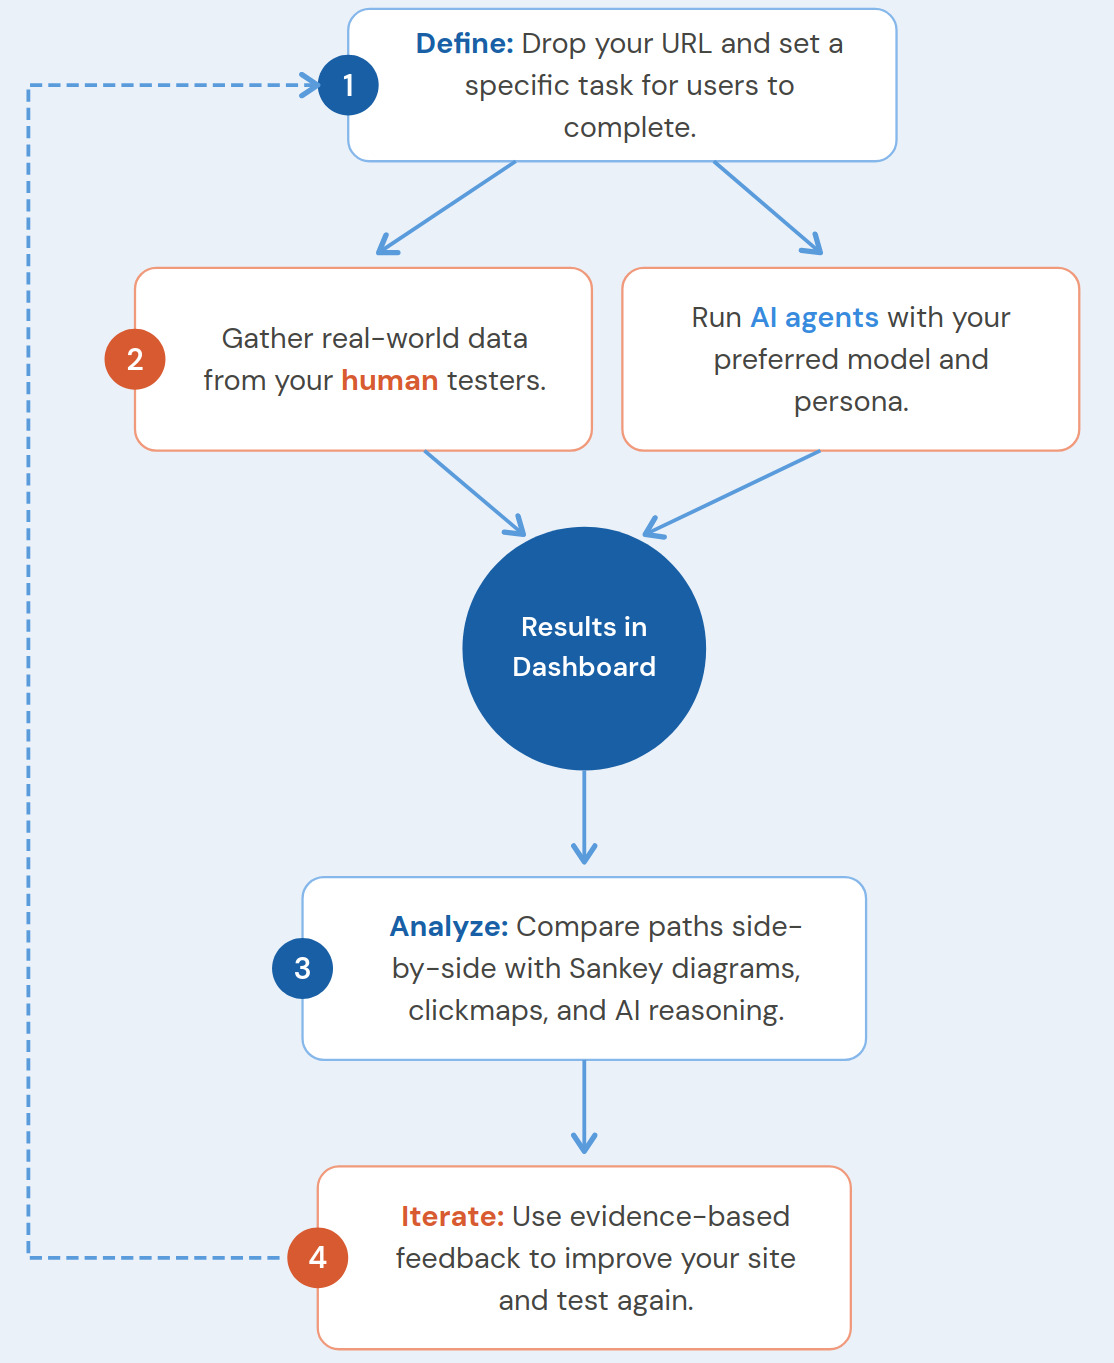
\includegraphics[width=\linewidth, height=30cm, keepaspectratio]{images/overview_image.jpeg}%
}

% (kept for reference but no longer used in layout)
\def\workflowdiagram{%
\begin{center}
\scalebox{0.55}{%
\begin{tikzpicture}[x=1cm, y=1cm,
  marrow/.style={
    ->, line width=0.18cm, color=CCblue,
    -{Stealth[length=0.55cm, width=0.42cm]}
  },
  harrow/.style={
    ->, line width=0.15cm, color=CChuman,
    -{Stealth[length=0.5cm, width=0.38cm]}
  },
  aarrow/.style={
    ->, line width=0.15cm, color=CCagent,
    -{Stealth[length=0.5cm, width=0.38cm]}
  },
  badge/.style={
    rectangle, rounded corners=0.35cm,
    fill=CCbluesoft, text=CCblue,
    font=\large\bfseries,
    inner xsep=0.45cm, inner ysep=0.18cm
  },
  annot/.style={font=\large, text=CCsec, align=center},
]
\begin{scope}[xshift=-1cm, yshift=-48cm]

% ── Create Project ────────────────────────────────────────────
\begin{scope}
  \clip[rounded corners=0.6cm] (3,83.5) rectangle (33,91.5);
  \fill[CCbluesoft] (3,89.8) rectangle (33,91.5);
  \fill[white] (3,83.5) rectangle (33,89.8);
\end{scope}
\draw[rounded corners=0.6cm, draw=CCborder, line width=0.06cm]
  (3,83.5) rectangle (33,91.5);
\foreach \dx in {1.1, 1.8, 2.5} {
  \fill[CCblue!35!white] (3+\dx, 90.65) circle (0.16cm);
}
\node[font=\Large, text=CCsec] at (18,87.8) {Enter site URL};
\node[font=\Large, text=CCsec] at (18,85.8) {Configure proxy};
\node[font=\LARGE\bfseries, text=CCdark, anchor=west] at (3,92.1)
  {Create Project};

% ── Arrow 1 → 2 ───────────────────────────────────────────────
\draw[marrow] (18,83) -- (18,81.5);

% ── Define Tasks ──────────────────────────────────────────────
\fill[CCbluesoft!40!white, rounded corners=0.25cm] (20,74.2) rectangle (28,80.2);
\draw[CCborder, line width=0.04cm, rounded corners=0.25cm] (20,74.2) rectangle (28,80.2);
\fill[CCblue!25!white, rounded corners=0.15cm] (22.5,79.7) rectangle (25.5,80.7);
\draw[CCborder, line width=0.03cm, rounded corners=0.15cm] (22.5,79.7) rectangle (25.5,80.7);
\foreach \y in {79.0, 78.1, 77.2, 76.3} {
  \draw[CCborder, line width=0.03cm] (20.8,\y) -- (27.4,\y);
}
\draw[CCblue!60, line width=0.04cm] (20.8,79.3) rectangle (21.3,79.8);
\draw[CCblue!60, line width=0.04cm] (20.8,78.4) rectangle (21.3,78.9);
\draw[CCblue, line width=0.06cm] (20.85,79.5) -- (21.0,79.7) -- (21.25,79.35);
\draw[CCblue, line width=0.06cm] (20.85,78.6) -- (21.0,78.8) -- (21.25,78.45);
\node[font=\Large, text=CCdark, anchor=west] at (2,78.8)
  {$\bullet$\quad Add task description};
\node[font=\Large, text=CCdark, anchor=west] at (2,76.8)
  {$\bullet$\quad Declare analysis points};
\node[font=\LARGE\bfseries, text=CCdark, anchor=west] at (1.5,81.0)
  {Define Tasks};

% ── Fork arrows ───────────────────────────────────────────────
\draw[harrow] (10,73.5) to[out=250, in=100] (5,71.5);
\draw[aarrow] (26,73.5) to[out=290, in=80]  (31,71.5);

% ── Human Testers card ────────────────────────────────────────
\begin{scope}
  \clip[rounded corners=0.6cm] (1,59) rectangle (17,71.5);
  \fill[CChumansoft] (1,70.0) rectangle (17,71.5);
  \fill[white] (1,59) rectangle (17,70.0);
\end{scope}
\draw[rounded corners=0.6cm, draw=CCborder, line width=0.06cm]
  (1,59) rectangle (17,71.5);
\foreach \dx in {1.0, 1.65, 2.3} {
  \fill[CChuman!40!white] (1+\dx, 70.75) circle (0.14cm);
}
\fill[CChumansoft] (4.5,67.8) circle (1.0cm);
\draw[CChuman, line width=0.12cm] (4.5,67.8) circle (1.0cm);
\fill[CChumansoft, rounded corners=0.5cm] (3.2,61.5) rectangle (5.8,66.6);
\draw[CChuman, line width=0.12cm, rounded corners=0.5cm] (3.2,61.5) rectangle (5.8,66.6);
\node[font=\large, text=CCdark, text width=9.5cm, align=left, anchor=north west]
  at (6.8,69.5) {%
  $\bullet$\ Gather human testers\\[5pt]%
  $\bullet$\ Share proxy link\\[5pt]%
  $\bullet$\ Log user demographics\\[5pt]%
  $\bullet$\ Record interactions%
};
\node[font=\LARGE\bfseries, text=CChuman, anchor=west] at (1,72.3)
  {Human Testers};

% ── AI Agent Runner card ──────────────────────────────────────
\begin{scope}
  \clip[rounded corners=0.6cm] (19,59) rectangle (35,71.5);
  \fill[CCagentsoft] (19,70.0) rectangle (35,71.5);
  \fill[white] (19,59) rectangle (35,70.0);
\end{scope}
\draw[rounded corners=0.6cm, draw=CCborder, line width=0.06cm]
  (19,59) rectangle (35,71.5);
\foreach \dx in {1.0, 1.65, 2.3} {
  \fill[CCagent!40!white] (19+\dx, 70.75) circle (0.14cm);
}
\fill[CCagentsoft, rounded corners=0.3cm] (20.7,67.0) rectangle (24.3,69.3);
\draw[CCagent, line width=0.12cm, rounded corners=0.3cm] (20.7,67.0) rectangle (24.3,69.3);
\fill[CCagent] (21.6,68.3) circle (0.30cm);
\fill[CCagent] (23.4,68.3) circle (0.30cm);
\fill[CCagentsoft!40!CCagent, rounded corners=0.1cm] (21.6,67.2) rectangle (23.4,67.6);
\fill[CCagentsoft, rounded corners=0.45cm] (20.4,61.5) rectangle (24.6,66.7);
\draw[CCagent, line width=0.12cm, rounded corners=0.45cm] (20.4,61.5) rectangle (24.6,66.7);
\fill[CCagent!20!white, rounded corners=0.2cm] (21.1,63.0) rectangle (23.9,64.8);
\draw[CCagent!50, line width=0.04cm, rounded corners=0.2cm] (21.1,63.0) rectangle (23.9,64.8);
\fill[CCagent] (21.7,63.9) circle (0.17cm);
\fill[CCagent!60] (22.5,63.9) circle (0.17cm);
\fill[CCagent!30] (23.3,63.9) circle (0.17cm);
\node[font=\large, text=CCdark, text width=9.5cm, align=left, anchor=north west]
  at (25.3,69.5) {%
  $\bullet$\ Configure agents\\[5pt]%
  $\bullet$\ Inject personality via system prompt\\[5pt]%
  $\bullet$\ VLMs + LLMs\\[5pt]%
  $\bullet$\ Let them run!%
};
\node[font=\LARGE\bfseries, text=CCagent, anchor=west] at (19,72.3)
  {AI Agent Runner};

% ── Arrows to Dashboard Analysis ──────────────────────────────
\draw[harrow] (9,59) to[out=300, in=90] (18,52.8);
\draw[aarrow] (27,59) to[out=240, in=90] (18,52.8);

% ── Dashboard Analysis card ───────────────────────────────────
\begin{scope}
  \clip[rounded corners=0.5cm] (7,48.2) rectangle (29,52.8);
  \fill[CCblue] (7,51.5) rectangle (29,52.8);
  \fill[white] (7,48.2) rectangle (29,51.5);
\end{scope}
\draw[rounded corners=0.5cm, draw=CCborder, line width=0.06cm]
  (7,48.2) rectangle (29,52.8);
\foreach \dx in {1.0, 1.65, 2.3} {
  \fill[white!60!CCblue] (7+\dx, 52.15) circle (0.15cm);
}
\node[font=\large\bfseries, text=white] at (18,52.15) {Dashboard Analysis};
\fill[CCbluesoft, rounded corners=0.06cm] (9.0,48.8) rectangle (10.0,50.9);
\fill[CCbluesoft, rounded corners=0.06cm] (10.4,49.3) rectangle (11.4,50.9);
\fill[CCblue!40!white, rounded corners=0.06cm] (11.8,48.6) rectangle (12.8,50.9);
\fill[CCblue!60!white, rounded corners=0.06cm] (13.2,49.1) rectangle (14.2,50.9);
\fill[CCblue] (19.5,50.0) circle (0.3cm);
\fill[white] (19.5,50.0) circle (0.12cm);
\fill[CChuman] (21.5,49.5) circle (0.3cm);
\fill[white] (21.5,49.5) circle (0.12cm);
\fill[CCagent] (23.5,50.2) circle (0.3cm);
\fill[white] (23.5,50.2) circle (0.12cm);

% ── Loop-back Re-evaluate arrow ───────────────────────────────
\draw[->, line width=0.15cm, color=CCblue, dashed,
      -{Stealth[length=0.5cm, width=0.38cm]}]
  (7,50.3) to[out=210, in=270] (0.5,64.0) to[out=90, in=240] (2.5,71.5);
\node[font=\large\bfseries, text=CCblue, rotate=90] at (1.8,64.0)
  {Re-evaluate};

\end{scope}
\useasboundingbox (0,0) rectangle (35cm,45cm);
\end{tikzpicture}%
}%
\end{center}
}


% ====================== 5. AGENT STEERING & EVALUATION =======================
\def\agentsteering{%
{\large \black
{\Large\bf Analysis \& Dashboard}\\[4pt]
{\bf $\bullet$\ Action Points}\\[3pt]
Task screenshots are annotated with glyphs marking where issues occur.
Each glyph links to an LLM-generated pain point with human and agent explanations and a matched recommendation.
Each action point routes to the most relevant visualisation for deeper analysis.\\[8pt]

{\bf $\bullet$\ Visualizations}\\[3pt]
Journey Flows (Sankey) $\cdot$ Click Heatmaps $\cdot$ Human vs.\ AI trajectory view.
Filterable by task and journey source.\\[12pt]

{\Large\bf Agent Steering \& HITL Re-evaluation}\\[4pt]
{\bf $\bullet$\ Alignment}\\[3pt]
Recorded human journeys are converted into prompt injections that steer agents toward human-like navigation patterns,
helping agents overcome complex scenarios. Steered and unsteered trajectories are compared in the Flow Chart view.\\[8pt]

{\bf $\bullet$\ Re-evaluation}\\[3pt]
Recorded human journeys enable re-evaluation via direct prompt-injection, mitigating the need for manual evaluation again and scaling up the process.
}%
}


% ====================== 6. CONCLUSION = Discussion ===========================
\def\conclusiontext{%
{\large \black
AI-driven automation benefits UX evaluation but requires alignment with human expectations.
Our HITL framework reduces the manual testing bottleneck while maintaining behavioral fidelity through trajectory-guided steering.
Agents are evaluated both with and without human steering, enabling measurement of alignment quality.
A remaining limitation is agent robustness on complex, dynamic webpages.
Future work targets tighter feedback loops and automated change propagation from action points to implementation.
}%
}


% ====================== REFERENCES ============================================
\def\bibfile{Poster-content}
\def\bibliotext{}
